\documentclass[onecolumn, draftclsnofoot,10pt, compsoc]{IEEEtran}
\usepackage{graphicx}
\usepackage{url}
\usepackage{setspace}
\usepackage{pstricks-add}
\usepackage{float}
\usepackage{soul}
\usepackage{color}

\usepackage{listings}


% COLOR DEFINITIONS FOR CODE LISTINGS
\definecolor{codegreen}{rgb}{0,0.6,0}
\definecolor{codegray}{rgb}{0.5,0.5,0.5}
\definecolor{codepurple}{rgb}{0.58,0,0.82}
\definecolor{backcolour}{rgb}{0.95,0.95,0.92}

\lstdefinestyle{mystyle}{
    backgroundcolor=\color{backcolour},
    commentstyle=\color{codegreen},
    keywordstyle=\color{magenta},
    numberstyle=\tiny\color{codegray},
    stringstyle=\color{codepurple},
    basicstyle=\footnotesize,
    breakatwhitespace=false,
    breaklines=true,
    captionpos=b,
    keepspaces=true,
    numbers=left,
    numbersep=5pt,
    showspaces=false,
    showstringspaces=false,
    showtabs=false,
    tabsize=2
}

\lstset{
	escapeinside={(*@}{@*)},
	style=mystyle
}

\usepackage{geometry}
\geometry{textheight=9.5in, textwidth=7in}

% 1. Fill in these details
\def \CapstoneTeamName{		AKA Robotics}
\def \CapstoneTeamNumber{		13}
\def \GroupMemberOne{     Arthur Shing}
\def \GroupMemberTwo{			Kevin Talik}
\def \GroupMemberThree{   Anish Asrani}
\def \CapstoneProjectName{		How to Make an Effective Robot Comedian}
\def \CapstoneSponsorCompany{	Oregon State University}
\def \CapstoneSponsorPerson{		Heather Knight}

% 2. Uncomment the appropriate line below so that the document type works
\def \DocType{		%Problem Statement
				%Requirements Document
				%Technology Review
				Design Document
				%Progress Report
				}

\newcommand{\NameSigPair}[1]{\par
\makebox[2.75in][r]{#1} \hfil 	\makebox[3.25in]{\makebox[2.25in]{\hrulefill} \hfill		\makebox[.75in]{\hrulefill}}
\par\vspace{-12pt} \textit{\tiny\noindent
\makebox[2.75in]{} \hfil		\makebox[3.25in]{\makebox[2.25in][r]{Signature} \hfill	\makebox[.75in][r]{Date}}}}
% 3. If the document is not to be signed, uncomment the RENEWcommand below
\renewcommand{\NameSigPair}[1]{#1}

%%%%%%%%%%%%%%%%%%%%%%%%%%%%%%%%%%%%%%%
\begin{document}

\bstctlcite{IEEEexample:BSTcontrol}
\begin{titlepage}
    \pagenumbering{gobble}
    \begin{singlespace}
        \hfill
        % 4. If you have a logo, use this includegraphics command to put it on the coversheet.
        %\includegraphics[height=4cm]{CompanyLogo}
        \par\vspace{.2in}
        \centering
        \scshape{
            \huge CS Capstone \DocType \par
            {\large\today}\par
            \vspace{.5in}
            \textbf{\Huge\CapstoneProjectName}\par
            \vfill
            {\large Prepared for}\par
            \Huge \CapstoneSponsorCompany\par
            \vspace{5pt}
            {\Large\NameSigPair{\CapstoneSponsorPerson}\par}
            {\large Prepared by }\par
            Group\CapstoneTeamNumber\par
            % 5. comment out the line below this one if you do not wish to name your team
            \CapstoneTeamName\par
            \vspace{5pt}
            {\Large
                \NameSigPair{\GroupMemberOne}\par
                \NameSigPair{\GroupMemberTwo}\par
                \NameSigPair{\GroupMemberThree}\par
            }
            \vspace{20pt}
        }
        \begin{abstract}
          To make an Effective Robot Comedian, we have developed three research questions to investigate our approach to designing this system: Adapting to audience response to humor, incorporating the crowd into the performance, and the effect of characterization in anthropomorphizing the robot. This paper outlines how our research questions will be incorporated into a system, and how we will study the shared space between a robot and an audience.
        \end{abstract}
    \end{singlespace}
\end{titlepage}
\newpage
\pagenumbering{arabic}
\tableofcontents
% 7. uncomment this (if applicable). Consider adding a page break.
%\listoffigures
%\listoftables
\clearpage

% 8. now you write!
\section{Overview}

\subsection{Scope}
	This research project is an investigation on developing and creating an effective robot comedian.
	This document is intended for communicating the purpose and planned design for the three areas of intended research.
	These areas include the development of the adaptive transitioning algorithm between jokes, the integration of an audience into the performance of a set, and the exploration of robotic character in joke content and delivery.
	As this document is intended for designing a research project, processes may differ from conventional development project designs.


\subsection{Purpose}
	This document describes the design and roadmap for the development of the robot comedian. The design is subject to change and will be revised as development progresses. Findings or limitations in the developmental process may influence the overall design of the product.

\subsection{Intended Audience}
	This document is intended for stakeholders and developers in the research project \textit{How to Make an Effective Robot Comedian}.

	% The first section covers the adaptation algorithm, the components of a stand-up set, and audience response comprehension. The next section explains "crowd-work", and how we will examine the influence of incorporating the audience into the robot's performance. Finally, the last section will cover the diversity of being a robot comedian, and how the qualities of a robot characterize the comedian.

\section{Adaptation}
\subsection{Goal}
  We hypothesize that to make the set the most effective, the comedian needs to transition to topics dependent on the audience response. The goal of this portion of the project is to determine if adapting the content from the audience response will enhance the overall performance of the comedian. Primarily, this algorithm needs to choose an optimal joke to fill the performance, while taking the audience into account.
\subsection{Methods}
In the beginning of the set, the comedian will present an "initialization" procedure, known as the "Seed Jokes" to test the response of the audience to different jokes. Depending on their response, the comedian will transition to a theme that is evaluated to be the best fit. The robot comedian will have many jokes to choose from that contain different material, but not all audiences will like all of the jokes. Figure 1 shows how the theme will be chosen from a set of up to \textit{k} themes. From the Seed Jokes, one of the themes will be chosen. The closing jokes set will be a subset of all jokes. These jokes might be stronger jokes than some of the others, and is helpful in ending the show on a stronger note. It may be a stretch to optimize with traditional machine learning because there may not be a large enough data set to adequately return results.

\begin{figure}[H]
  \centering
  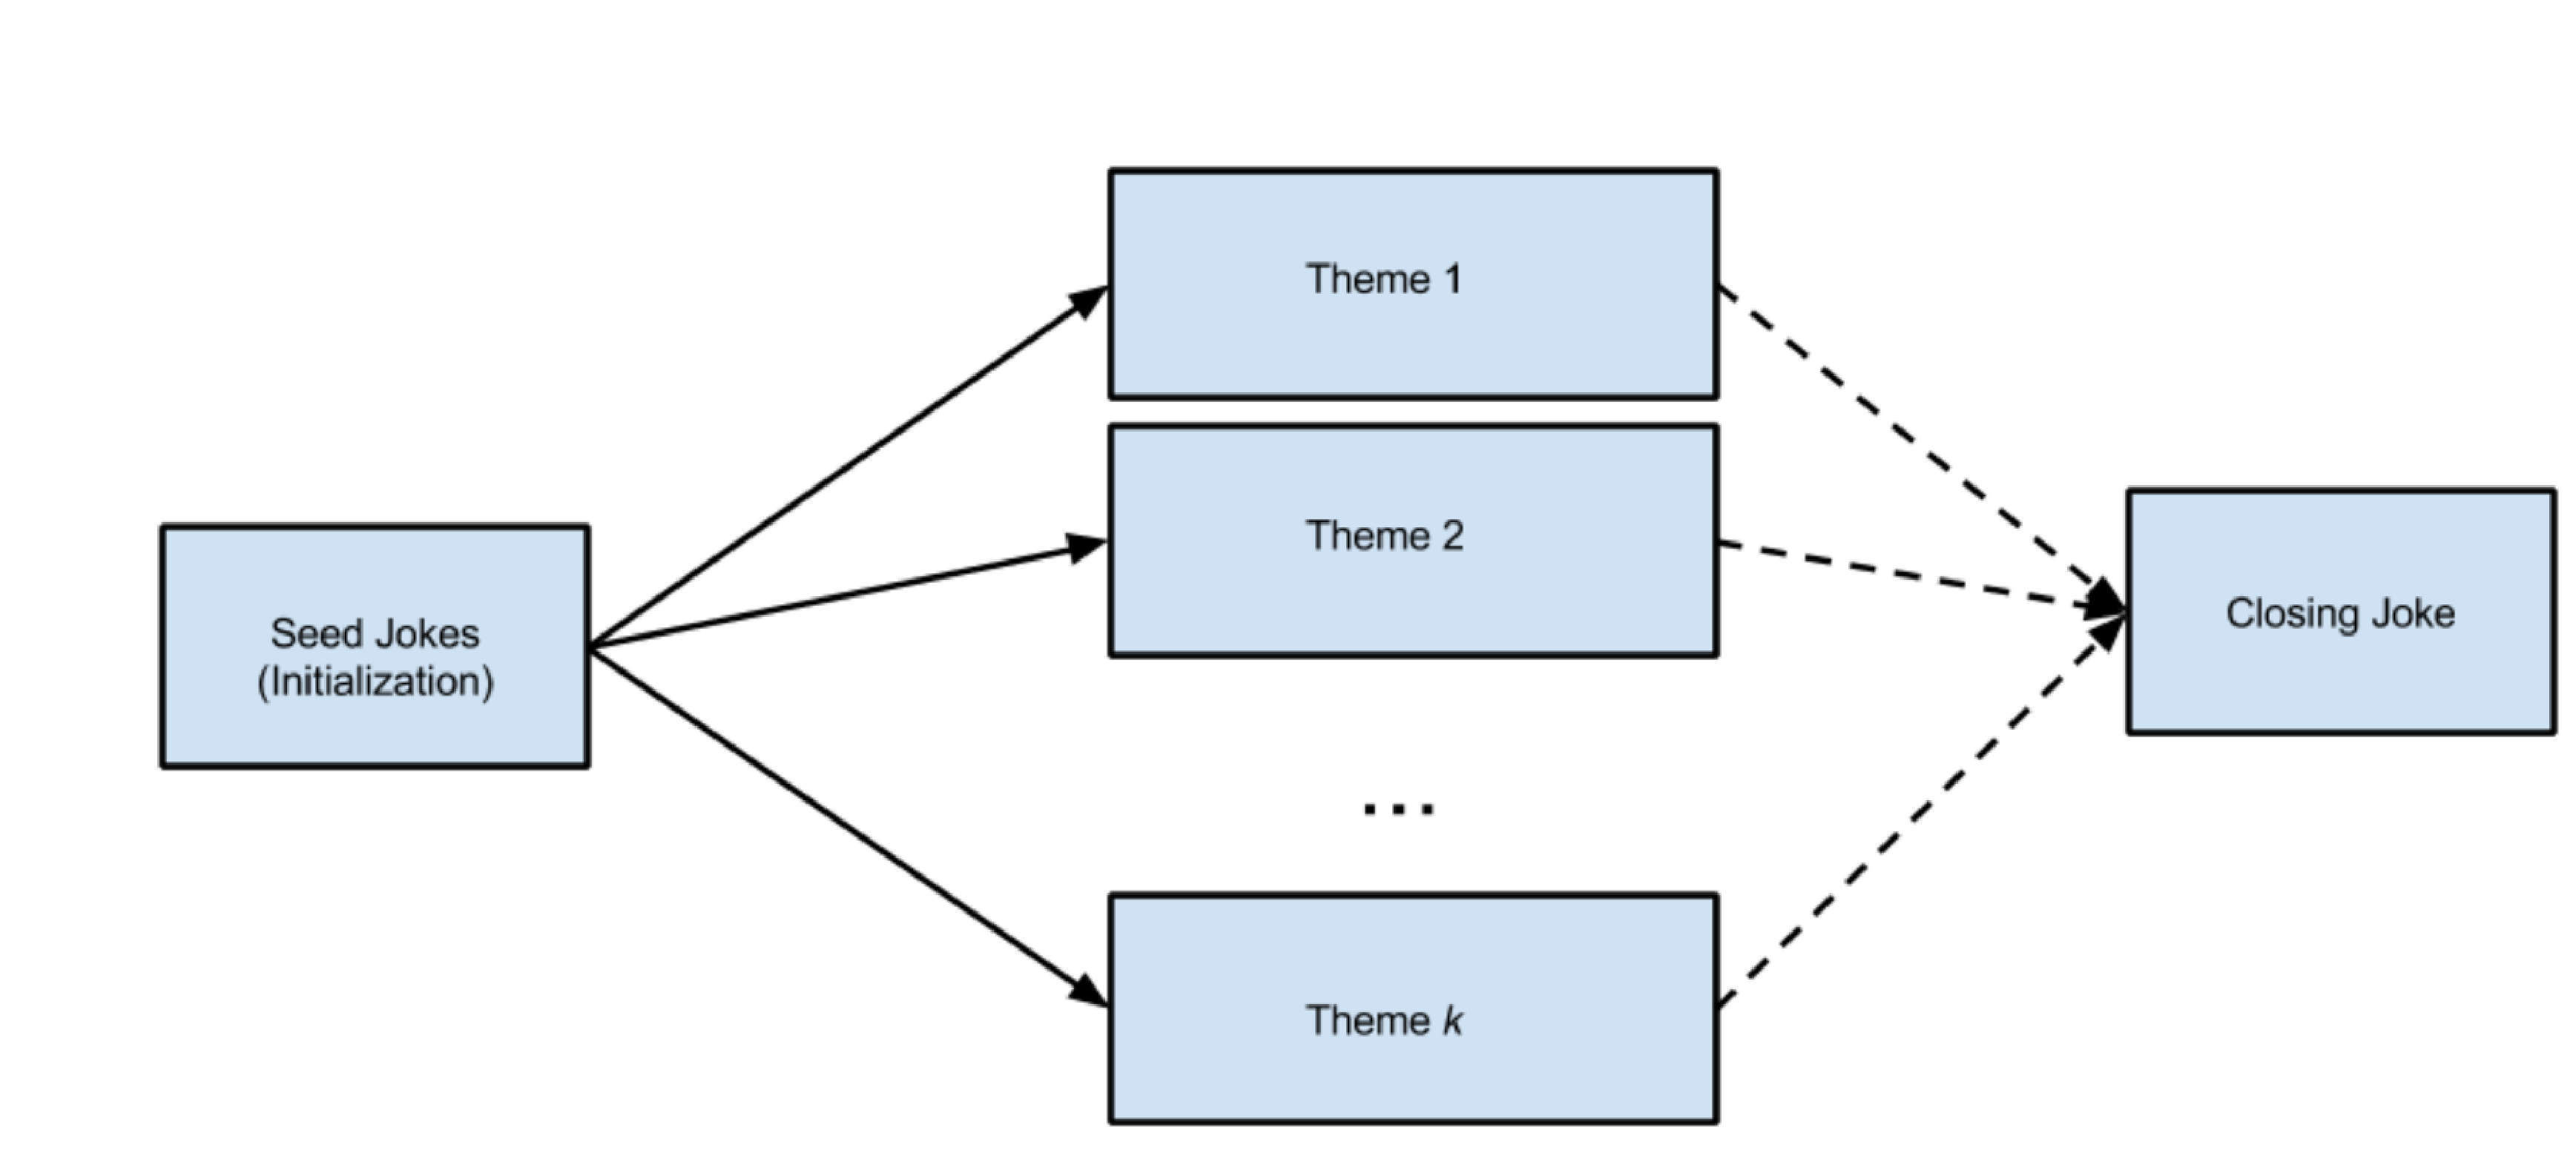
\includegraphics[width=0.75\textwidth,height=0.75\textheight,keepaspectratio]{fig0}
  \caption{This shows how the algorithm will have up to \textit{k} Themes to choose from, determined from the seed joke. The closing joke is a subset of the set of all jokes, and may be outside of a specific theme. There could be different spanning trees of performances that end at the same closing joke}
\end{figure}

Figure 2 depicts how a joke will be represented by the robot. It will perform the joke, collect audience feedback information, and branch to the joke that will best fit the response. For example, if two of the seed jokes are about "food" and "Mindfulness", the performance will branch to the respective theme that matches the audience response (Branch 1 "Food" or Branch 2 "Mindfulness"). If jokes with a theme of "food" are not landing with the audience, the algorithm will need to know when to transition to a new theme, or when to end the set. When the robot tells a joke, it needs to be able to analyze the feedback and choose the next joke to perform. This needs to be done quickly, so that the robot is not spending noticeable time (for the audience) choosing a joke. There may not be a lot of jokes to choose from, but the choice needs to be made fast.

\begin{figure}[H]
  \centering
  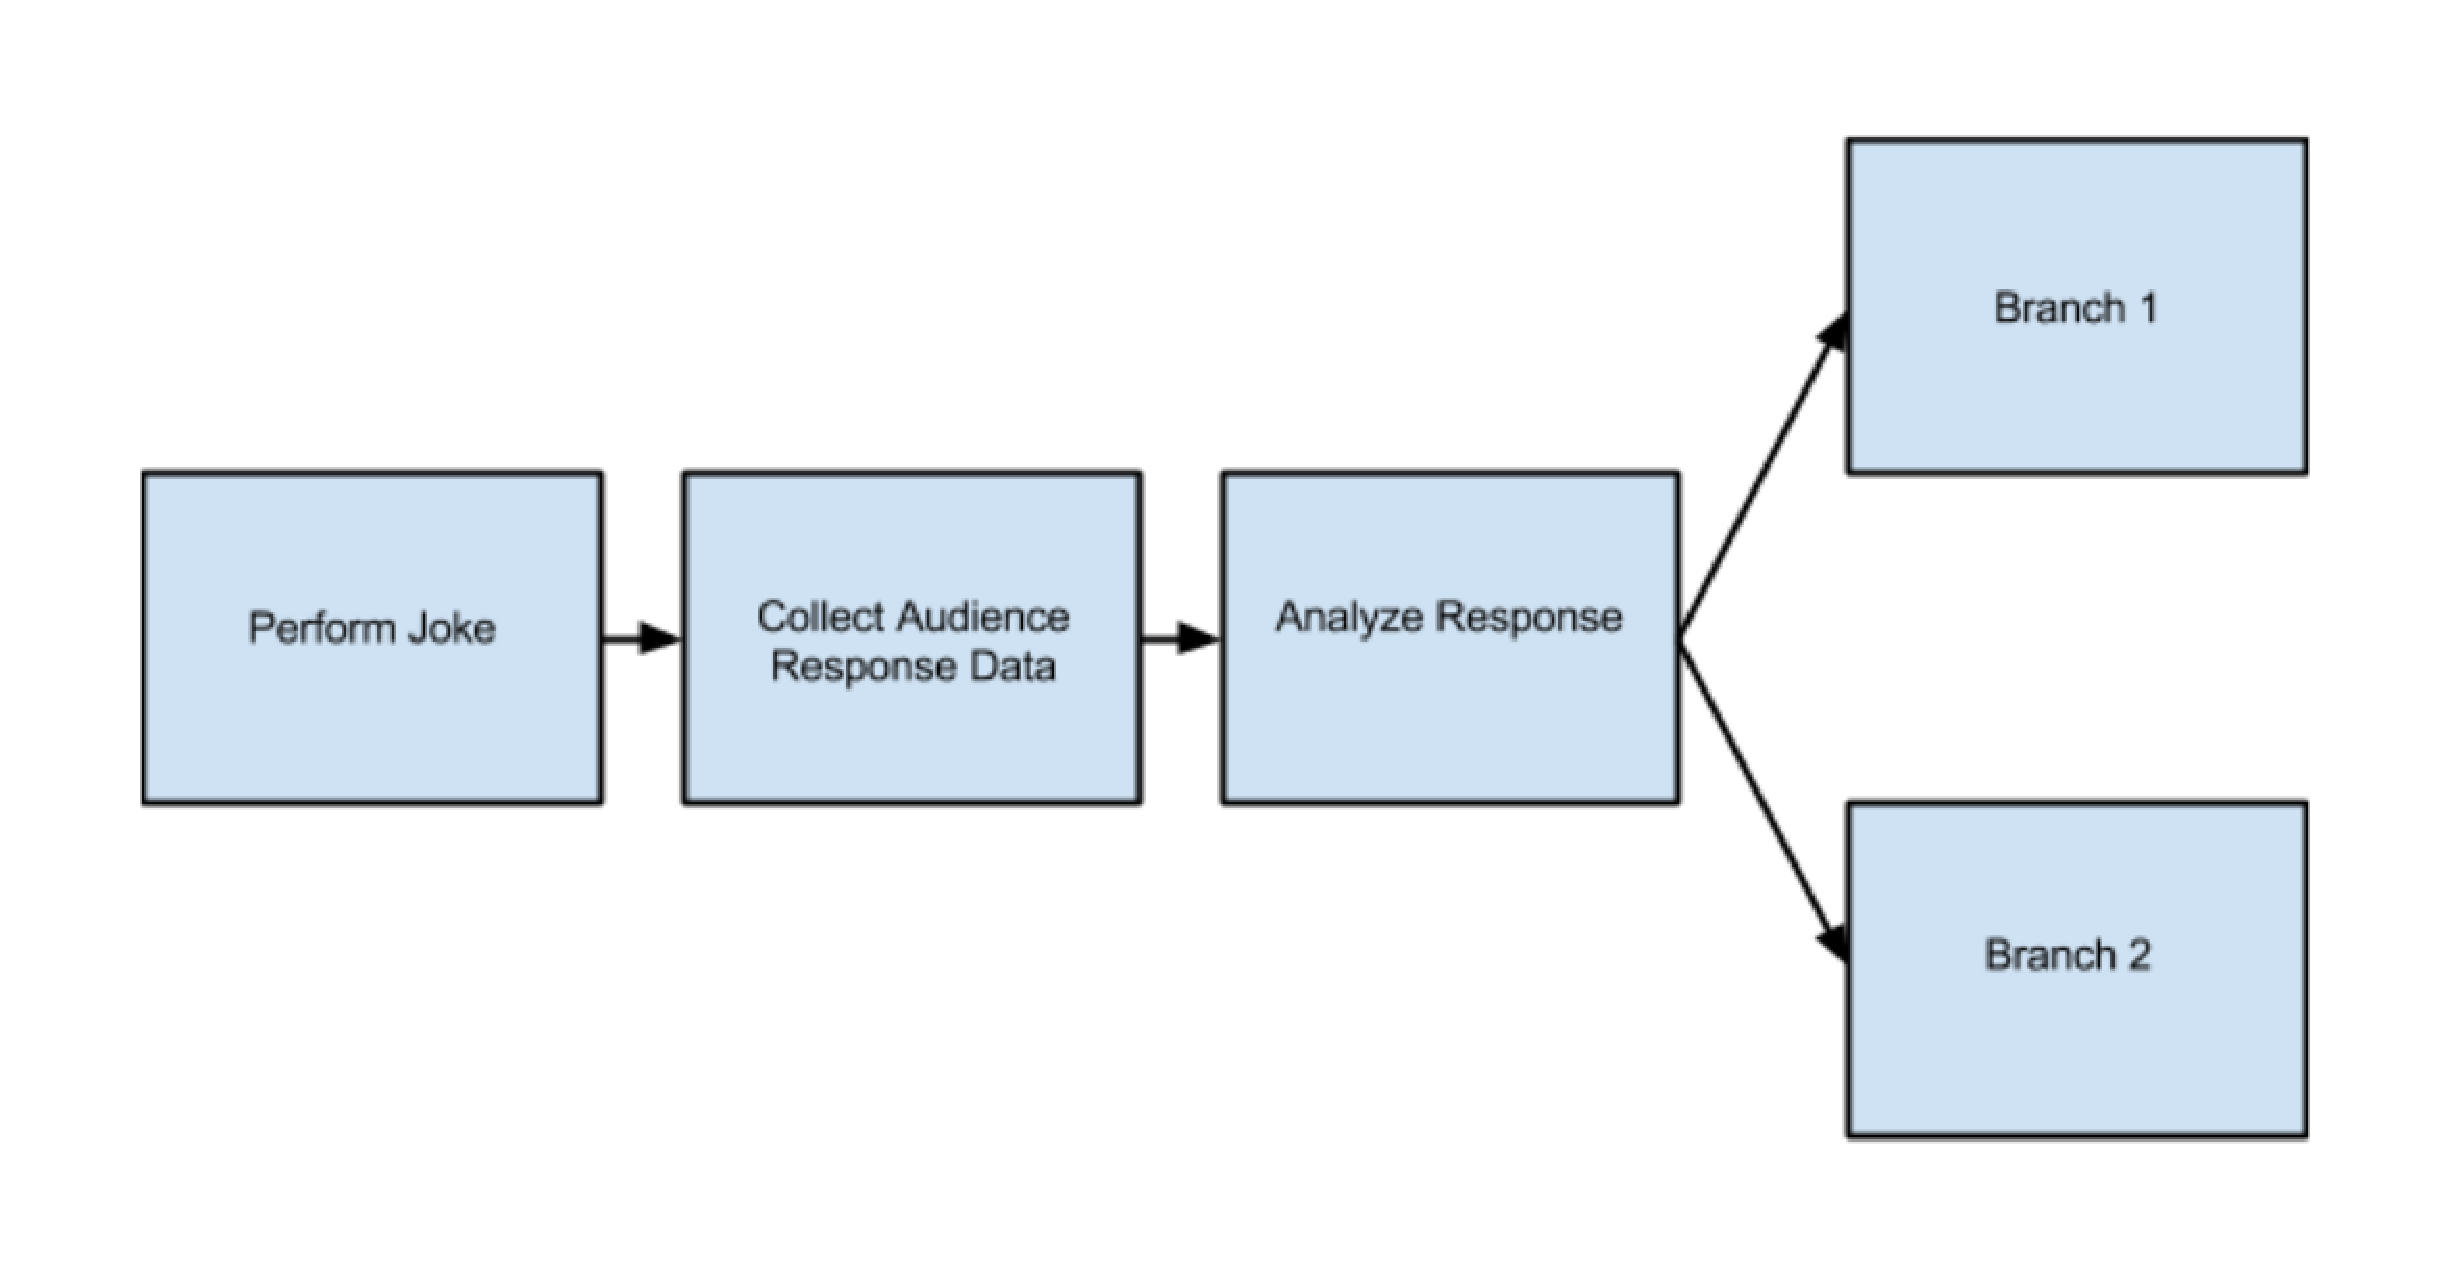
\includegraphics[width=0.75\textwidth,height=0.75\textheight,keepaspectratio]{fig1}
  \caption{ This flow-chart depicts how, once the robot delivers a joke, will wait for feedback, interpret data, and then make a joke decision (Branch 1 and Branch 2)}
\end{figure}

Generally, the performance will have three parts: the Seed Jokes, the Middle Content, and the Closing Joke. This adaption algorithm will determine the transitions between all of these parts and the jokes they consist of. The Seed will influence the Middle Content (which will be chosen themed jokes and basis of the show). The Middle Content will transition to the Closing Joke when it is time to end the show. This final joke needs to reflect the performance that the robot gave. The most work that needs to be done is learning about closing jokes, and their influence on the performance and difference between other jokes


\section{Crowd-work}
Crowd-work in a performance involves incorporating the audience and making them feel like they are a part of the show. This can be done in different ways -  calling out and talking to the audience, listening to the audience and making relevant comments, asking them questions to keep them engaged. We want to analyze the importance of this crowd-work in a robot stand-up comedy performance.

There are various degrees of this crowd-work we want to test. The first one would be no crowd-work whatsoever. The robot goes about performing its set while acknowledging its lack of sensing and interaction. The robot does not directly address the audience at all.

The second would be over-the-top and inaccurate crowd-work. The robot will talk to the audience directly but it will be completely wrong in its observation.The absurdity of a robot trying to understand the audience and being completely off could be entertaining for the audience, or it may not connect with the audience at all. The exact reception of this sort of crowd-work is something we are trying to study.

The third way would be realistic but pre-meditated. Some pre-known facts about the audience will be built into the robot. These pre-known facts could include the location of the performance, age demographics of the audience. For example, if the audience is known to be college-aged, the robot will be fed input to make comments about things relevant to college students.

The fourth would be actually looking for cues from the audience during certain situations. This would be done by asking certain questions and capturing words from the audience and using the same word in a comment later,  For example, the robot could ask a simple question about the weather, or the audience member's hometown. The robot can listen for specific words and ask another question about that specific town or city. Another cue that the robot will look for is audience volume levels after the delivery of jokes. The robot will keep track of the audience input. The robot could then acknowledge if the audience enjoyed the joke or did not enjoy the joke using these inputs.

These methods will be used to check to what degree is crowd-work important for a robot. Since crowd-work and interaction are "human" behaviors, the audience's response will be used to see if they enjoy a humanized robot or if they prefer a more robotic one, or maybe even a combination of both.


\section{Character}
\subsection{Goal}
In Jerry Palmer's \textit{Taking Humor Seriously}, comic meaning is argued to depend on the interrelated factors of a joke's context and setting, its delivery, the identity of the deliverer, and the audience \cite{Palmer:1993}.
Of specific interest to us are the factors of a joke's delivery and the identity of the deliverer.
In previous studies, robot comedy has been used to analyze effective aspects of joke delivery.
However, little has been done in discovering effective aspects of a joke's content as it relates to the identity of the deliverer.
For example, Sj\"{o}bergh and Araki \cite{RobotsMakeThings:2008} found that jokes were perceived as funnier when delivered by a robot, rather than being delivered in text form.
Sj\"{o}bergh and Araki used word-play jokes that were gathered from the internet, and delivered them through a robot by using a flat, machine-like sounding text-to-speech tool called AquesTalk.
While Sj\"{o}bergh and Araki did not implement measures for analyzing non-verbal delivery, other work has examined the importance of non-verbal signals in delivering jokes \cite{KatevasRobot:2014} \cite{KnightEightLessons:2011}.
Despite this, there is little to no existing literature on the effectiveness of jokes related to the identity of the deliverer.
In our context, this means examining the effectiveness of robot-specific jokes in robot comedy.
The goal of this section of the project is to examine whether or not robot comedy can benefit from having jokes delivered from a robot's perspective.

\subsection{Methods}
To address this goal, jokes will be written from a human or robot perspective.
The jokes written from a human perspective will have a corresponding robot version, ideally with as much one-to-one correspondence as possible, where possible.
These jokes will be subject to intense scrutiny by members of the project and by the client, such that revisions and edits can be made to create funny jokes with a definite correspondence between the two versions.
For example, a human version of a joke might look like the following. Lines with a definite correspondence with the robot version are highlighted.

\begin{lstlisting}
Hey, hey, I got news. This is big.
Ok, quiet down. Get this.
That's RIGHT folks.
I'm no longer single. *throws hands up*
(*@  \hl{I met a man on tinder.}  @*)
(*@  \hl{His name's Sebastian. He's a math nerd.}  @*)
(*@  \hl{Swiped right as fast as my fingers could move.}  @*)
\end{lstlisting}

The robot version of the above joke is shown below.

\begin{lstlisting}
Hey, hey, I got news. This is big.
Ok, quiet down. Get this.
That's RIGHT folks.
I'm no longer single. *throws hands up*
(*@  \hl{I met a robot on tinder. }  @*)
(*@  \hl{His name's Data.  He's a really geeky robot.}  @*)
(*@  \hl{Swiped right as fast as my motors could turn.}  @*)
\end{lstlisting}

\subsection{Development process of joke writing}
These jokes will be scripted in Choregraphe, where adjustments to vocal tones and pausing will be made.
Then, animating the robot for non-verbal gestures will be done to enhance the delivery.
The overall process may look similar to Figure \ref{fig:write_process}.

\begin{figure}[H]
  \centering
  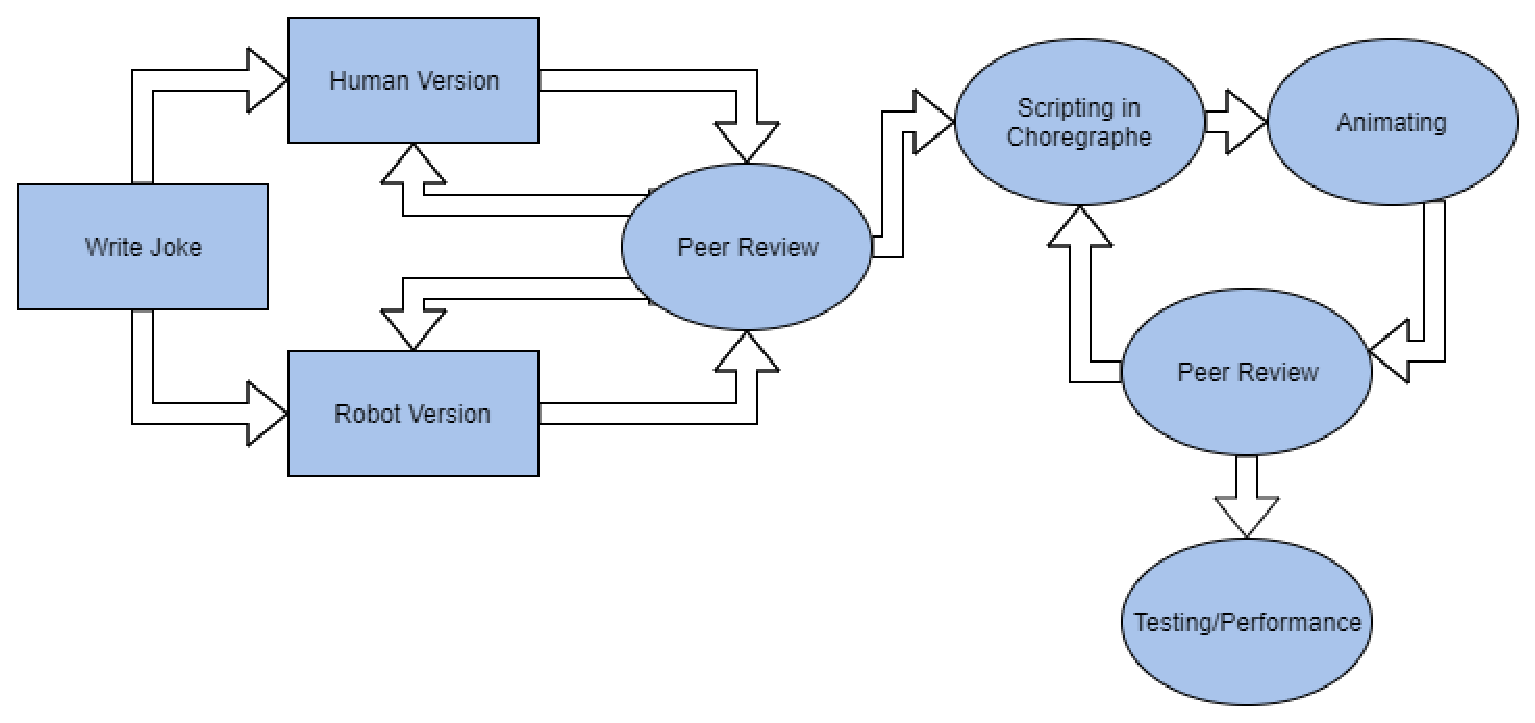
\includegraphics[width=0.75\textwidth,height=0.75\textheight,keepaspectratio]{joke_writing_process}
  \caption{The work flow from joke writing to testing.}
	\label{fig:write_process}
\end{figure}

\section{Conclusion}
  Designs for the adaptive transitioning algorithm between jokes, the integration of an audience into the performance of a set, and the exploration of robotic character in joke content and delivery have been described. These designs are subject to change and revision. In following through with this in the research and development process, we hope to create an effective robot comedian.



\pagebreak

\pagebreak
\clearpage
\section{Glossary}
\begin{description}
  \item [Algorithm] \hfill \\ The software program that receives input to make an optimized choice; in this project, the algorithm is in context to the adaptation program.
	\item [Animating] \hfill \\ The NAO robot can be programmed to animate and move while speaking. This can be used to improve non-verbal communication between the robot and the audience.
  \item [API] \hfill \\ Application Programming Interface
  \item [Branch] \hfill \\Looking at the graph (edges and nodes) of a performance, a branch is a decision choice made by the algorithm.
  \item [Choregraphe] \hfill \\ Software used to program behavior and performance sets, made by SoftBank Robotics
  \item [Closing Joke] \hfill \\The final joke in a performance; this is helpful if it is a successful joke to end on a good note.
  \item [Crowd-work] \hfill \\ Part of a Comedian's performance that involves content from the current audience
  \item [NAO] \hfill \\ Model of Robot that will be used as the Comedian Agent, made by SoftBank Robotics
  \item [SoftBank Robotics] \hfill \\ Manufacturer of the NAO robot, NAOqi API, and Choregraphe software
  \item [Seed Jokes] \hfill \\ Set of three jokes that initialize the adaptation algorithm.
  \item [Set] \hfill \\Short for "Stand-up" set; this may also be used to describe to the collection of jokes: "A Set of Jokes"
  \item [Tree] \hfill \\This is the path through the set of jokes the algorithm took during a performance

\end{description}

\bibliographystyle{IEEEtran}
\bibliography{refs}

\end{document}
